\subsection{Preprocessing}

\subsubsection{Data Cleaning} 

    3.2.1.1 Handling null values. During the preprocessing phase, one of the important steps to was to address the null values, particularly within the \texttt{Income} column. Several solutions were considered for dealing with the null values in this column. 

    First, it was proposed to fill null values with the median of their respective groups. This method imputes missing values with the meadian income of similar groups based on other features, such as \texttt{Education} or \texttt{Marital\_Status}. But after examining the relationship between \texttt{Income} and these categorical variables, we observed weak correlations:
        - For \texttt{Education} levels, the correlation coefficients ranged from -0.200576 to 0.081552 which indicate a weak relationship between these features.
        - Similarly, for \texttt{Marital\_Status}, the correlation coefficients ranged from -0.025843 to 0.0031706, also suggesting a weak relationship between these features.

    Given these weak correlations, imputing null values based on the meadian of their respective groups might not provide a meaninful impact on the models. It may also introduce inaccuracies into the dataset because neither \texttt{Education} nor \texttt{Marital Status} strongly predict \texttt{Income}. After testing this approach, the F1 scores of Logistic Regression, SVM, Decision Trees, and K-Nearest Neighbors significantly decreased with 0.045786, 0.04433, 0.149474, and 0.099193, respectively, less in scores.

    Second, another approach for these missing \texttt{Income} values was to fill it with 0. This method can be justified if a null value represents customers; lack of income. However, this assumption is generally not accurate for most of the datasets. It could significantly skew the data distribution and inflate the count of customers' with zero income. Therefore, filling null values with zero was viewed as not optimal due to its potential to misrepresent the information of the customers in the dataset. The only model that decreased in F1 score using this approach is the Decision Tree which resulted in 0.036149 less in score.

    Lastly, given the drawbacks of the first two approaches, it was decided to remove rows with null values. This decision was made by considering the analysis done in the features and preserving the integrity of the data. Although this approach may result in a smaller dataset, it ensures that reliability and complete information, which reduces the potential for skewed results and maintain data quality.

    3.2.1.2 Handling Outliers. Outliers were observed within the \texttt{Income}, \texttt{Mnt.*}, and \texttt{Num.*} columns during the exploratory data analysis phase. Visualization tools, such as kernal density estimate and scatter plots, indicated the presence of extreme values that could potentially affect the modelling. The following algorithm for removing outliers on continuous variables was implemented:

\begin{figure}[H]
    \centering
    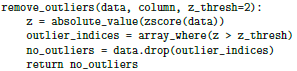
\includegraphics[width=\linewidth]{figures/removing_outliers.png}
    \caption{Removing Outliers}
    \label{fig:income hist}
\end{figure}

    By applying this algorithm, it ensures that the analysis is not skewed by extreme values, leading to more accurate results and improves the quality of the models.

\subsubsection{Feature Engineering}

    3.2.2.1 Creating Total Children Feature. A new column called \texttt{Total\_Children} was created by summing up the \texttt{Kidhome} and \texttt{Teenhome} columns. This new feature provides anothger information for the total number of children in each customer's household, which could help in understanding the purchasing behavior or creating new marketing strategies based on this new feature.

    3.2.2.2 Removing Unrealistic Customers based on Year of Birth. During the exploratory data analysis phase, a number of outliers in the \texttt{Year\_Birth} column was recognized, that is why the dataset was filtered to only include records where the column value is 1940 or later. This ensures a realistic age range for customers.

    3.2.2.3 Converting dates to Datetime and validation. The values in the \texttt{Dt\_Customer} column was converted to a datetime type. To ensure the dataset contains valid dates, checks were implemented to verify that there are no future dates and that the year of birth is not later than the year of becoming a customer.

    3.2.2.4 Calculating Days Since Becoming a Customer. The number of days since the date of becoming a customer up to the current date was calculated. This new feature, \texttt{Days\_Since\_Customer}, was created to help in understanding the customer tenure, which can be important in models to predict customer loyalty.

    3.2.2.5 Cleaning Marital Status Values. There are two approaches proposed in cleaning these values. At first, dropping the rows with \texttt{Marital\_Status} values of \texttt{YOLO}, \texttt{Absurd}, and \texttt{Alone} was considered. However, this approach may possibly negatively affect the integrity of the data. It also resulted to a lesser F1 scores in SVM and Decision Tree models with a result of 0.027663 and 0.027541, respectively, less in scores.
    
    That is why replacing this status labels with \texttt{Single} was done to maintain data size and integrity. This homogenization helps in reducing the variability within the data. This helps in decreasing the number of different values which can help in making the analysis more straightforward.

\subsubsection{One-Hot Encoding}

Columns \texttt{Education} and \texttt{Marital\_Status} are categorical values. While there is an option to use factorization for these data, there is a risk of misinterpretation since the factorized values could imply that one number has a greater value than the other, which could lead to misinterpreation during the modelling process. 

\subsubsection{Interaction Features}

Given the statistical evidence from the ANOVA test - F = 2.815 for \texttt{Kidhome} and F = 4.461 for \texttt{Teenhome}, with p-values well below the 0.05 significance level - during the explroatory data analysis phase, the results shows strong evidence that \texttt{Marital\_Status} significantly impacts the number of children and teenagers in a household. This suggests that marital status may interact with household composition that may provide a meaningful impact on the model. To quanitify these relationship, interaction features were created by multiplying each one-hot encoded marital status column by \texttt{Kidhome} and \texttt{Teenhome} to create new interaction columns. These interaction features can potentially imrpove the performance of the models. They allow models to provide deeper insights on how households interact with the customers' marital status.

There were discontinued approaches using interaction feature between \texttt{Total_Children} and one-hot encoded \texttt{Marital_Status} because during the exploratory data analysis phase, 

\subsubsection{Feature Selection}

The objective was to construct a predictive model to classify customers who might purchase the new year-end sale offer based on variables that may have a direct or indirect impact. Through careful analysis, there are columns that were dropped, such as \texttt{ID}, \texttt{Dt\_Customer}, \texttt{Kidhome}, and \texttt{Teenhome}. 

The \texttt{ID} contains unique identifiers for each record which are typically irrelevant to the outcome of predictive models. The date when the customer joined have been used to derive new feature, \texttt{Days\_Since\_Customer}, therefore the original date is no longer necessary for the modelling. The columns \texttt{Kidhome} and \texttt{Teenhome} were used to create interaction features and new feature, \texttt{Total\_Children}. Retaining these original columns might be redundant and could even introduce noise.

Additionally, interaction features were introduced by  using one-hot encoded marital status and variables like \texttt{Kidhome} and \texttt{Teenhome}. Removing the original one-hot encoded columns can help in avoiding multicollinearity and potentially improve the performance of the models due to reduced dimensionality and complexity.

\subsubsection{Scaling}

Large distance between features can negatively affect the model's performance. For example, the \texttt{Income} value are in thousands, while the other variab;es, especially those that have underfone one hot encoding only range in single digits. With the use of feature scaling, this would help the models in dealing with values that are too distant in range.

The use of \texttt{StandardScaler} helps prepare the dataset for many machine learning algorithms, particularly those sensistive to the scale of features, such as Support Vector Machines (SVM), and K-Nearest Neighbors (KNN). 

\subsubsection{Polynomial Feaures}

While adding more features to a model doesn't equate to better performance, there is still a significant effect to a machine learning model when utilized correctly. The introduction of polynomial features would create a polynomial based on a single feature where each monomial would become an input in the model. The use of \texttt{interaction\_only=True} extends the datset with features that represent the products of pairs of original features. This is based on assumption that the relationship between some variables could exhibit boosting when combined. By integrating polynomial feature, it can help the models with a comprehensive framework capture more complex relationships within the data.

